\section{Introduction}
$K$-mer counting is a seemingly relatively straightforward process. Given a sequence $X = \{x_1,\dots,x_L\}$ of length $L$, for each position $i\in 1\leq i\leq \left(L-k+1\right)$ within the sequence, a sub-string is sliced from $[i,i+k)$. Where ``[" indicates inclusion, and ``)" indicates non-inclusive. A hash-map, or dictionary as known within Python, then saves the count for each $k$-mer as encountered in $X$. In many applications, the frequency of each $k$-mer would be calculated by dividing each $k$-mer count by the total number of $k$-mers, \emph{i.e.} $L-k+1$. 

SEEKR differs from this approach in that the algorithm adjusts from the non-uniformity of $k$-mers within our genome. Some $k$-mers are more, or less, frequent than others solely due to mononucleotide frequencies within the genome. Therefore, the enrichment for already common $k$-mers, or depletion of rare $k$-mers, are not informative unless it is known if they are significantly more enriched than background. To account for this, SEEKR calculates a $z$-score for each $k$-mer rather than a frequency.

The $z$-score is calculated by first calculating the $k$-mer frequencies within some reference set of sequences, \emph{e.g.} the transcriptome. From this reference set of $k$-mer frequencies, the mean frequency of each $k$-mer $\mu_j$ and the standard deviation of each $k$-mer $\sigma_j$ is calculated. 

For each $k$-mer frequency $j$ within a sequence $X$, $X_j$ has a $z$-score $X^*_j$: 

\begin{equation}
    X_j^* = \frac{X_j-\mu_j}{\sigma_j}
    \label{eq:zscore}
\end{equation}


We observed when studying the $k$-mer similarities between XIST and RSX that these $z$-scores were approximately log-normally distributed. For the analysis within that paper, we transformed $z$-scores as outlined in 2.X.X. However, we sought to perform a more rigorous analysis of different methodologies for adjusting $k$-mer counts. This chapter outlines the methods that we used and their results. 

\begin{figure}[h]
\centering
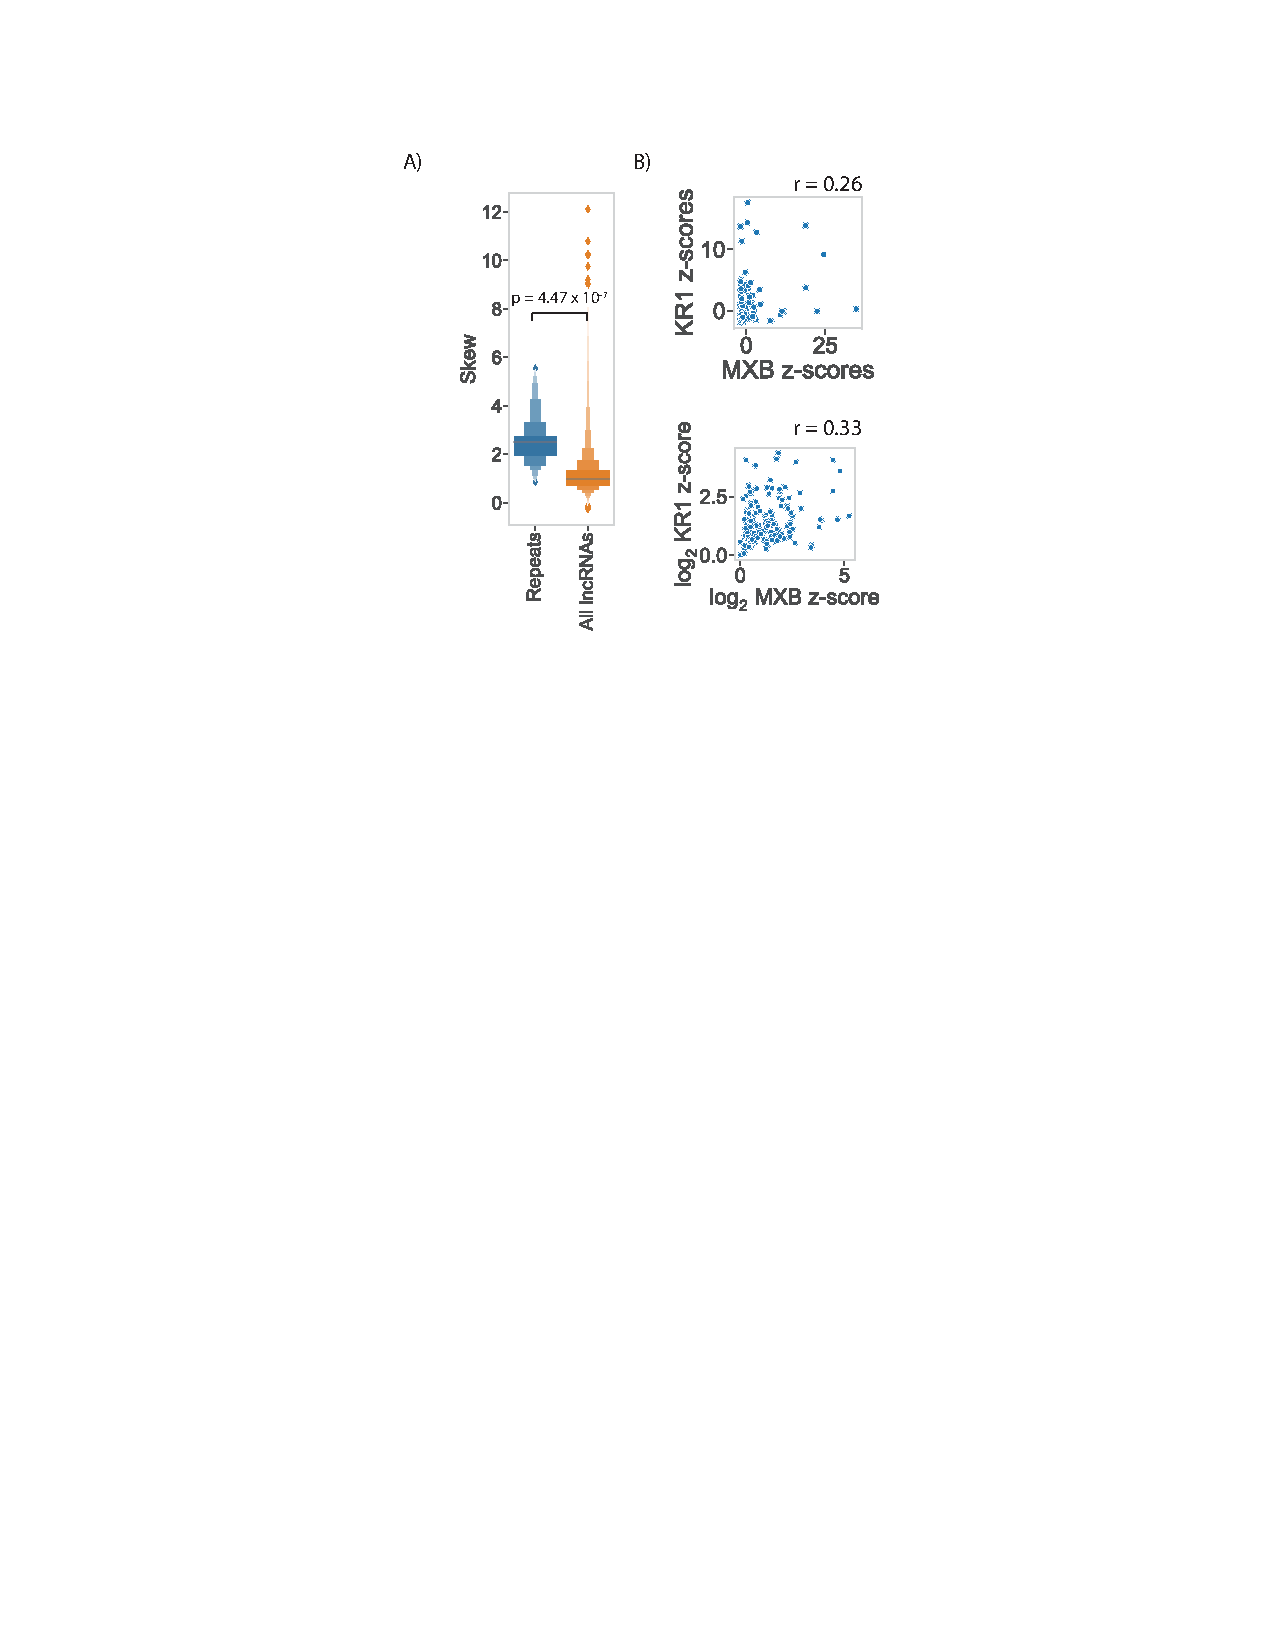
\includegraphics[width=\textwidth]{images/kmerskew.pdf}
\caption{Xist and Rsx repeats and the set of reference GENCODE lncRNAs have $z$-score vectors with positive (right) skew; $z$-scores in Xist and Rsx are significantly more skewed than those in there reference set of GENCODE lncRNAs (Mann-Whitney U Test). B) Representative plots of improvement in correlation from untransformed (top) and log-transformed $z$-scores (bottom).}
\label{fig:skew}
\end{figure}